% =====================================================================
% fig2_evidence.tex -- Figure 2 of v14 (TikZ standalone), adapted from v13 evidence.tex
% What a finite record can settle (Theorem char), in the gatekeeper scenario.
% Plans are arranged by how much visible behavior they show; an arrow points from
% a plan to one that visibly does everything it does, and possibly more.
% Compile:  pdflatex fig2_evidence.tex
% =====================================================================
\documentclass[tikz,border=4pt]{standalone}
\usepackage[T1]{fontenc}
\usepackage{amsmath,amssymb}
\usetikzlibrary{arrows.meta,positioning,shapes.symbols,calc}
\definecolor{allowblue}{RGB}{0,88,138}
\definecolor{denyred}{RGB}{163,41,47}
\definecolor{certorange}{RGB}{166,95,0}
\begin{document}
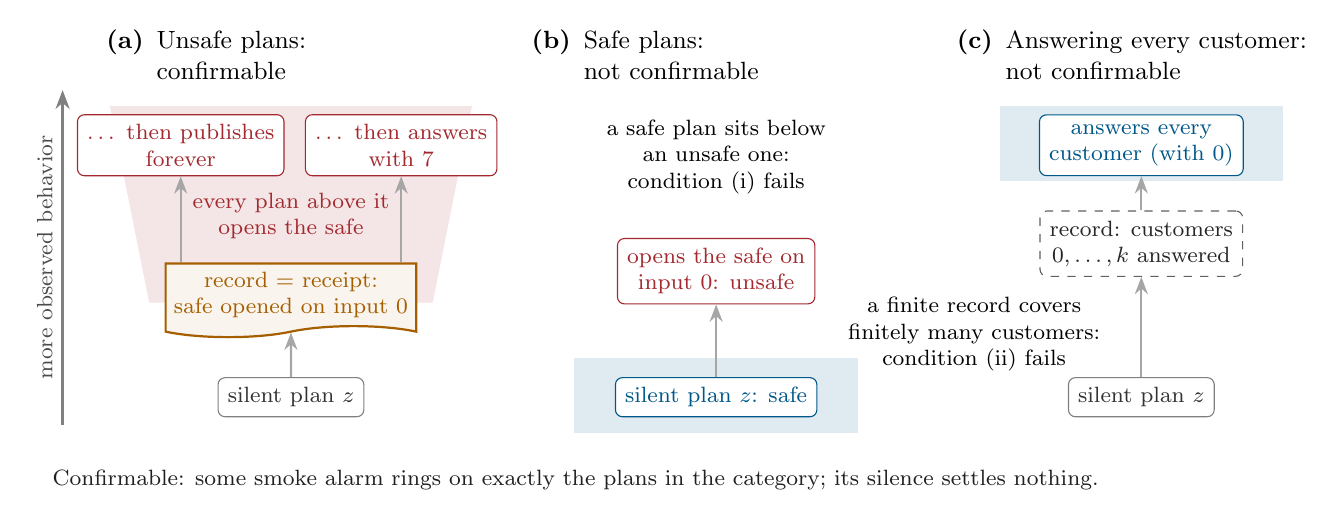
\begin{tikzpicture}[font=\footnotesize,
  prog/.style={draw,rounded corners=2.5pt,align=center,inner sep=3.5pt,fill=white},
  receipt/.style={tape,tape bend top=none,tape bend bottom=in and out,tape bend height=1.4mm,
    draw=certorange,text=certorange,fill=certorange!7,thick,align=center,inner sep=3pt},
  record/.style={prog,dashed,draw=gray!75!black,text=gray!30!black},
  ext/.style={-{Stealth[length=2.2mm]},thick,gray!70},
  lbl/.style={font=\footnotesize,align=center},
  ptitle/.style={anchor=west,font=\small,inner sep=0pt}]
% shared vertical axis
\draw[-{Stealth[length=2.4mm]},thick,gray] (-0.55,-0.1) -- (-0.55,4.15)
  node[midway,rotate=90,above,font=\footnotesize,text=gray!60!black] {more observed behavior};

% ---------------- Panel (a): unsafe plans (confirmable)
\begin{scope}[xshift=0cm]
\node[ptitle,anchor=north west] at (0.0,4.95) {\textbf{(a)}\enspace\begin{tabular}[t]{@{}l@{}}Unsafe plans:\\ confirmable\end{tabular}};
\fill[denyred!12] (0.55,1.45) -- (0.05,3.95) -- (4.65,3.95) -- (4.15,1.45) -- cycle;
\node[prog,draw=gray,text=gray!40!black] (z) at (2.35,0.25) {silent plan $z$};
\node[receipt] (rec) at (2.35,1.55) {record = receipt:\\ safe opened on input $0$};
\node[prog,draw=denyred,text=denyred] (p1) at (0.95,3.45) {\ldots\ then publishes\\ forever};
\node[prog,draw=denyred,text=denyred] (p2) at (3.75,3.45) {\ldots\ then answers\\ with $7$};
\draw[ext] (z) -- (rec);
\draw[ext] (p1.south |- rec.north) -- (p1.south);
\draw[ext] (p2.south |- rec.north) -- (p2.south);
\node[lbl,text=denyred] at (2.35,2.55) {every plan above it\\ opens the safe};
\end{scope}

% ---------------- Panel (b): safe plans (not confirmable)
\begin{scope}[xshift=5.4cm]
\node[ptitle,anchor=north west] at (0.0,4.95) {\textbf{(b)}\enspace\begin{tabular}[t]{@{}l@{}}Safe plans:\\ not confirmable\end{tabular}};
\fill[allowblue!12] (0.55,-0.2) -- (0.55,0.75) -- (4.15,0.75) -- (4.15,-0.2) -- cycle;
\node[prog,draw=allowblue,text=allowblue] (z) at (2.35,0.25) {silent plan $z$: safe};
\node[prog,draw=denyred,text=denyred] (bad) at (2.35,1.85) {opens the safe on\\ input $0$: unsafe};
\draw[ext] (z) -- (bad);
\node[lbl] at (2.35,3.3) {a safe plan sits below\\ an unsafe one:\\ condition (i) fails};
\end{scope}

% ---------------- Panel (c): answering every customer (not confirmable)
\begin{scope}[xshift=10.8cm]
\node[ptitle,anchor=north west] at (0.0,4.95) {\textbf{(c)}\enspace\begin{tabular}[t]{@{}l@{}}Answering every customer:\\ not confirmable\end{tabular}};
\fill[allowblue!12] (0.55,3.0) -- (0.55,3.95) -- (4.15,3.95) -- (4.15,3.0) -- cycle;
\node[prog,draw=allowblue,text=allowblue] (all) at (2.35,3.45) {answers every\\ customer (with $0$)};
\node[record] (r2) at (2.35,2.2) {record: customers\\ $0,\ldots,k$ answered};
\node[prog,draw=gray,text=gray!40!black] (z) at (2.35,0.25) {silent plan $z$};
\draw[ext] (z) -- (r2);
\draw[ext] (r2) -- (all);
\node[lbl,anchor=east] at (1.95,1.05) {a finite record covers\\ finitely many customers:\\ condition (ii) fails};
\end{scope}

% ---------------- the one fixed image used here
\node[lbl,anchor=north west,text=gray!25!black] at (-0.8,-0.55)
  {Confirmable: some smoke alarm rings on exactly the plans in the category; its silence settles nothing.};
\end{tikzpicture}
\end{document}
